\documentclass[aspectratio=169]{beamer}
% \usetheme{Madrid}
% package to use double spacing
\usepackage{setspace}

\usepackage{tikz}

% % neural network
% \usetikzlibrary{matrix,chains,positioning,decorations.pathreplacing,arrows}



% package to add wrapfigure
\usepackage{wrapfig}


% package to add graphs
\usepackage{pgfplots}

% packages to add images
\usepackage{graphicx}

% stuff for checkerboard
\usetikzlibrary{matrix.skeleton}
\tikzstyle{ball} = [circle, shading=ball, minimum size=1cm]
\newcommand{\bl}{\node [ball, ball color=black!80!white, draw=black!65!white, thin]{};}
\newcommand{\wh}{\node [ball, ball color=white] {};}

% stuff for decision trees
\usepackage{forest}

\tikzset{
	Midway/.style={
  midway,
  above,
  font=\scriptsize,
  text width=1.5cm,
  align=center,
  },
Above/.style={
  midway,
  above,
  font=\scriptsize,
  text width=1.5cm,
  align=center,
  },
Below/.style={
  midway,
  below,
  font=\scriptsize,
  text width=1.5cm,
  align=center
  }
}

% Titular Information
	\title[NN and GA To Play Draughts] % (optional, only for long titles)
	{Playing Draughts using Neural Networks and Genetic Algorithms}
	\author[T. Nguyen] % (optional, for multiple authors)
	{Thien Nguyen}
	\institute[Durham] % (optional)
	{
	Department of Computer Science\\
	Durham University
	}
	\subject{Computer Science}
% ------------------------------

% Plan for 8 minutes.

	% A title slide: Project title, student name, course, date
	%  An outline: What are the elements of your talk?
	% A problem description, possibly both informal and formal
	% Motivation: Why do you want to solve this problem? Previous work, and how it relates to what you are doing
	% Your approach to solving the problem
	% What you have accomplished so far (not relevant for marking!) Analysis: How will you judge the outcome of your work?
	% A conclusion slide: What did or will you accomplish?
	% What still needs to be done
\begin{document}
\pgfplotsset{compat=1.15}

% Title Frame
\frame{\titlepage}

% Outline Page
\begin{frame}

  \frametitle{Outline}
  %Content goes here
	%An outline: What are the elements of your talk?
	\begin{block}{Problem Description}
		% This is important information
	 \end{block}
	\begin{block}{Motivation}
	% This is important information
	\end{block}
	\begin{block}{Related Work}
	% This is important information
	\end{block}
	\begin{block}{Approach}
	% This is important information
	\end{block}
	\begin{block}{Curent Progress}
	% This is important information
	\end{block}
	\begin{block}{Conclusion}
		% This is important information
	\end{block}
	  
	%  \begin{alertblock}{This is an Alert block}
	%  This is an important alert
	%  \end{alertblock}
  
	%  \begin{exampleblock}{This is an Example block}
	%  This is an example 
	%  \end{exampleblock}
\end{frame}

% Problem Description
\begin{frame}
	\frametitle{Why Draughts?}
	\begin{figure}[ht!]
		\centering
		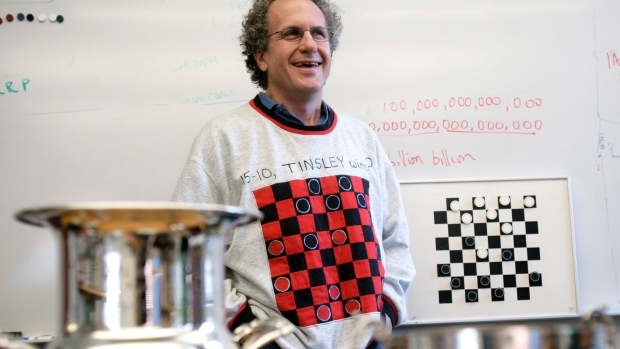
\includegraphics[width=80mm]{schaeffer.jpg}
		\caption{Schaeffer literally brute forced Checkers in 2007. \cite{schaeffer_solving_1996}}
	\end{figure}
\end{frame}

\begin{frame}
  \frametitle{Problem Description}
	\framesubtitle{A problem in Computer Science (..before AlphaZero existed)}
	% \setlength{\parindent}{4em}
	\setlength{\parskip}{1.5em}
	% More content goes here
	% Why is it important?
	% Currently (except for AlphaGo Zero) are really good at exploiting human games and definining "intuition" from there.

	Presently, A variety of Draughts AI players tend to be designed to play at a fixed ability.
	\par
	While it has produced very competitive and intelligent players, they require human  intervention in order to improve their performance.
	\par
	% This is due to their dependency on pre-defined move databases, where optimal moves are pre-calculated, and recalled when necessary. \\
	By combining Neural Networks and Genetic Algorithms, this issue could possibly be solved by creating a player that can grow in ability over time, without the dependency on move-banks.


\end{frame}

% Motivation
\begin{frame}
	\frametitle{Motivation}
	\framesubtitle{Why have I chosen to tackle this?}
	% Why do you want to solve this problem? Previous work, and how it relates to what you are doing
	%More content goes here

	\begin{itemize}
		\item Enjoyed AI Search Submodule
		\item Interested in seeing whether genetic algorithms are still relevant
		\item Interested in machine learning
		\item ..I like board games
	\end{itemize}

	% Interested in neural networks, really enjoyed AI Search submodule. Inherent competitiveness against peers
	% Not necessarily interested in solving something new; also not expected for a bachelors degree.
\end{frame}

% Related Work
\begin{frame}
	\frametitle{Related Work}
	\framesubtitle{Similar works of art but no cigar}
	% Why do you want to solve this problem? Previous work, and how it relates to what you are doing
	\begin{block}{Samuel (59')}
		Uses Genetic Algorithms to improve coefficents of a set of heuristics to evaluate Draughts games. \cite{samuel_studies_2000}
	\end{block}
	%More content goes here
	\begin{block}{Blondie24 (97')}
		Uses an Evolutionary Algorithm and Neural Networks to evaluate Draughts games. (Quite similar!) \cite{chellapilla_evolving_1999}
	\end{block}

	 \begin{block}{Giraffe (15')}
		Uses contemporary machine learning techniques to train a Neural Network to evaluate Chess games. \cite{lai_giraffe:_2015}
	 \end{block}

	 \begin{block}{Uber (Last month)}
		Uses genetic algorithms to train convolutional neural networks to play Atari Games. \cite{such_deep_2017}
	 \end{block}
	% Interested in neural networks, really enjoyed AI Search submodule. Inherent competitiveness against peers
	% Not necessarily interested in solving something new; also not expected for a bachelors degree.
\end{frame}

% Current Approach
\begin{frame}
	\frametitle{Current Approach}
	% Your approach to solving the problem
	\framesubtitle{How will I tackle this; in a nutshell}
	% Why do you want to solve this problem? Previous work, and how it relates to what you are doing
	%More content goes here
	\begin{itemize}
		\item Evaluate a checkerboard state
		\item Choose the best move for a given state
		\item Generate a population of agents
		\item Determine good agents from the population
		\item Make better agents from the good ones
	\end{itemize}

\end{frame}

% ----------------------------
% Neural Networks
% ----------------------------

	% Example Checkers Game
	\begin{frame}
		\frametitle{Evaluating Checkerboards}
		\begin{figure}[ht!]
			\centering
			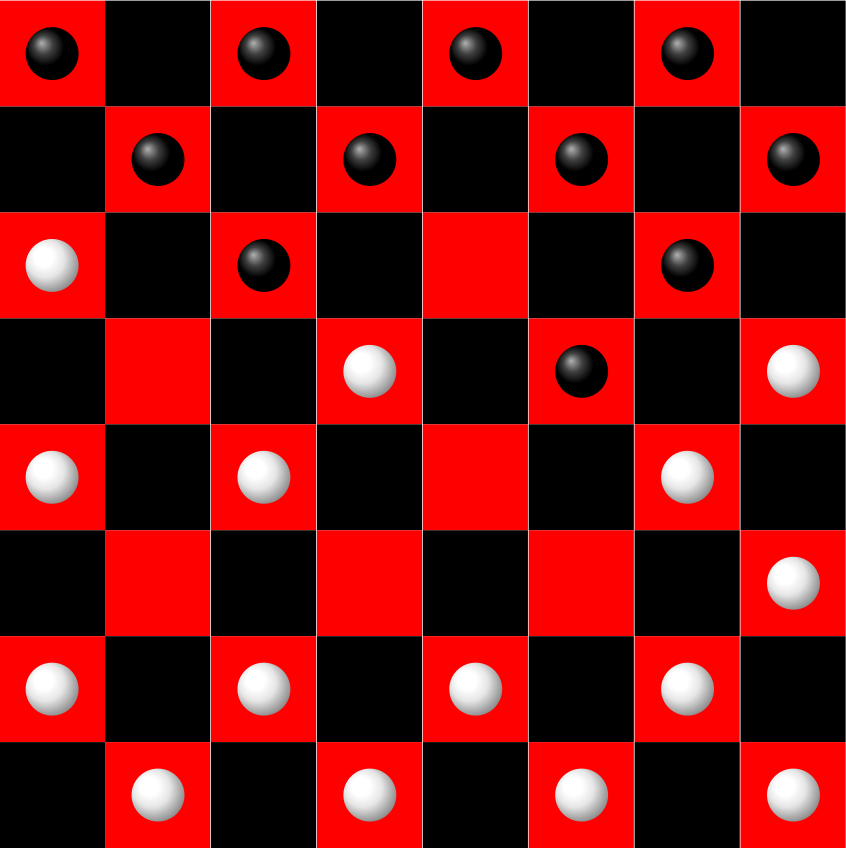
\includegraphics[width=50mm]{sampleGame.png}
			\caption{An example state of a checkerboard. \label{overflow}}
		\end{figure}
	\end{frame}

	% Example Neural Network Frame
	\begin{frame}
		\frametitle{Neural Networks}
		\begin{figure}
			\tikzset{%
				every neuron/.style={
					circle,
					draw,
					minimum size=0.9cm
					},
				neuron missing/.style={
					draw=none, 
					scale=4,
					text height=0.333cm,
					execute at begin node=\color{black}$\vdots$
				},
			}

			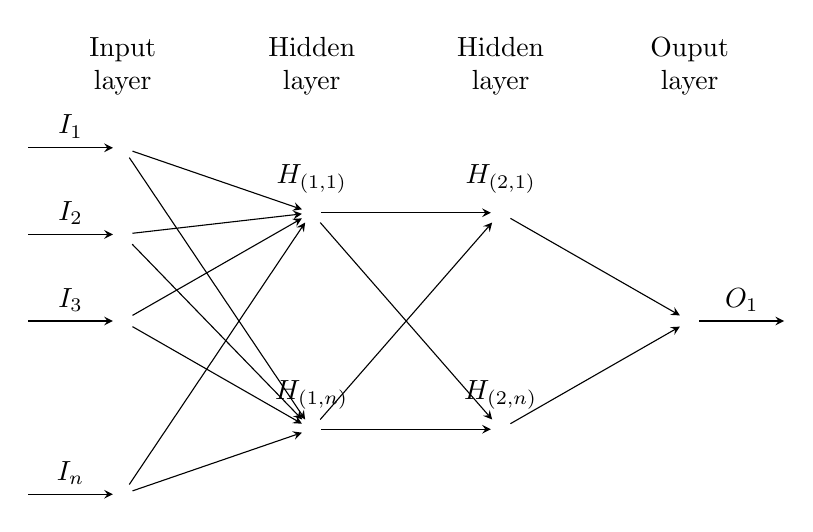
\begin{tikzpicture}[x=1.2cm, y=1.1cm, >=stealth]

			% draw nodes
				% % input values
				% \foreach \m/\l [count=\y] in {1,2,3,missing,4}
				% 	\node [every neuron/.try, neuron \m/.try] (input-\m) at (-0.5,2.5-\y) {};

				% input layer
				\foreach \m/\l [count=\y] in {1,2,3,missing,4}
				\node [every neuron/.try, neuron \m/.try] (input-\m) at (0,2.5-\y) {};
				
				% layer 1
				\foreach \m [count=\y] in {1,missing,2}
				\node [every neuron/.try, neuron \m/.try ] (hidden1-\m) at (2,2-\y*1.25) {};

				% layer 2
				\foreach \m [count=\y] in {1,missing,2}
				\node [every neuron/.try, neuron \m/.try ] (hidden2-\m) at (4,2-\y*1.25) {};

				% output layer
				\foreach \m [count=\y] in {1}
				\node [every neuron/.try, neuron \m/.try ] (output-\m) at (6,0.5-\y) {};

			% input layer
			\foreach \l [count=\i] in {1,2,3,n}
				\draw [<-] (input-\i) -- ++(-1,0)
				node [above, midway] {$I_{\l}$};

			% hidden 1
			\foreach \l [count=\i] in {{(1,1)},{(1,n)}}
				\node [above] at (hidden1-\i.north) {$H_{\l}$};

			% hidden 2
			\foreach \l [count=\i] in {(2,1),(2,n)}
				\node [above] at (hidden2-\i.north) {$H_{\l}$};

			% output layer
			\foreach \l [count=\i] in {1}
				\draw [->] (output-\i) -- ++(1,0)
				node [above, midway] {$O_\l$};

			% lines from input to hidden 1
			\foreach \i in {1,...,4}
				\foreach \j in {1,...,2}
					\draw [->] (input-\i) -- (hidden1-\j);
			
			% lines from hidden 1 to hidden 2
			\foreach \i in {1,...,2}
			\foreach \j in {1,...,2}
				\draw [->] (hidden1-\i) -- (hidden2-\j);

			% lines from hidden 2 to putput
			\foreach \i in {1,...,2}
				\foreach \j in {1}
					\draw [->] (hidden2-\i) -- (output-\j);

			% headings
			\foreach \l [count=\x from 0] in {Input, Hidden, Hidden, Ouput}
				\node [align=center, above] at (\x*2,2) {\l \\ layer};

			\end{tikzpicture}
		\end{figure}
	\end{frame}

	% Checkerboard Outline
	\begin{frame}
		\frametitle{Checkerboard}
		\begin{figure}[ht!]
			\centering
			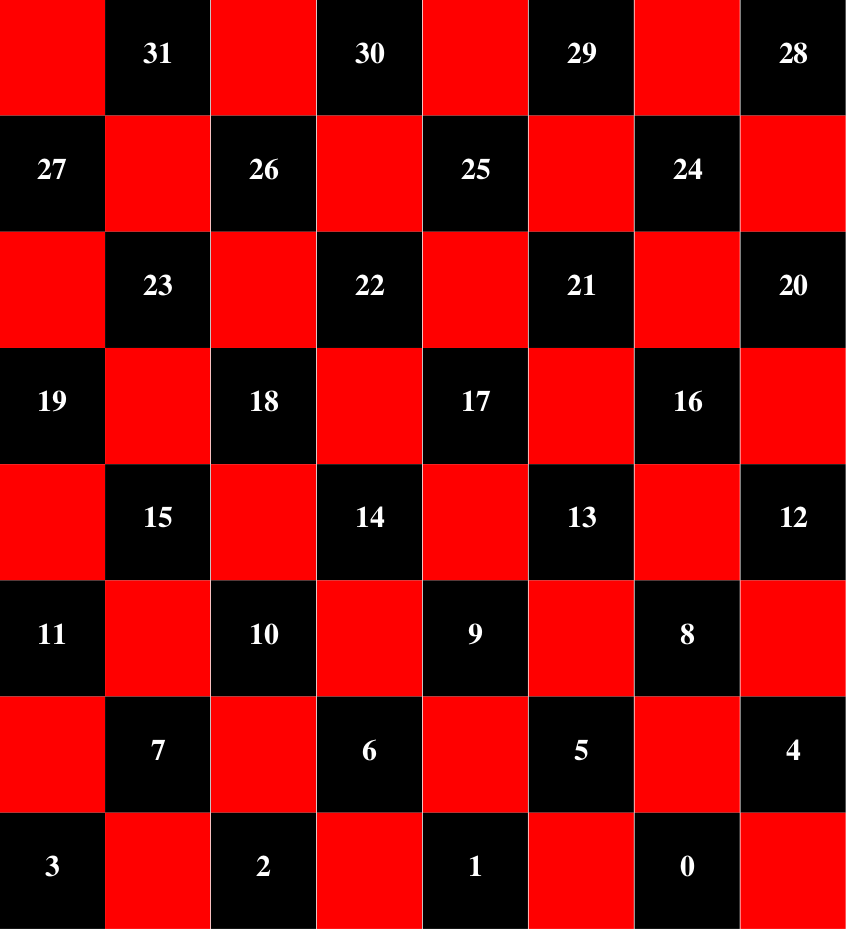
\includegraphics[width=50mm]{checkerboard.png}
			\caption{The indexes of the 32 pieces of the input layer are the immediate values of the positions on the board. \label{overflow}}
		\end{figure}
	\end{frame}

	% Applied Neural Network Diagram
	\begin{frame}
		\frametitle{Neural Networks}
		\begin{figure}
			\tikzset{%
				every neuron/.style={
					circle,
					draw,
					minimum size=0.9cm
					},
				neuron missing/.style={
					draw=none, 
					scale=4,
					text height=0.333cm,
					execute at begin node=\color{black}$\vdots$
				},
			}

			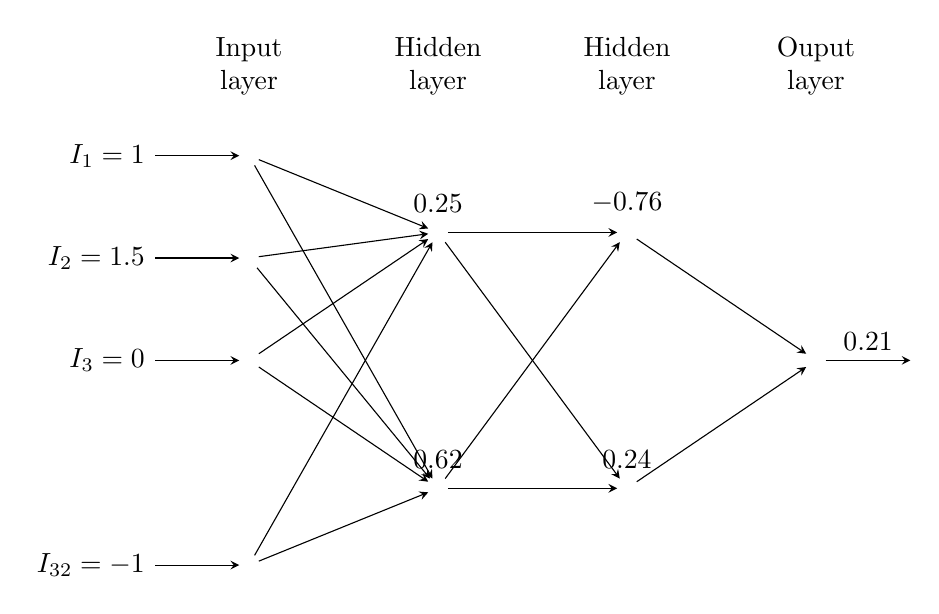
\begin{tikzpicture}[x=1.2cm, y=1.3cm, >=stealth]

					% input layer
					\foreach \m/\l [count=\y] in {1,2,3,missing,4}
					\node [every neuron/.try, neuron \m/.try] (input-\m) at (0,2.5-\y) {};
					
					% layer 1
					\foreach \m [count=\y] in {1,missing,2}
					\node [every neuron/.try, neuron \m/.try ] (hidden1-\m) at (2,2-\y*1.25) {};

					% layer 2
					\foreach \m [count=\y] in {1,missing,2}
					\node [every neuron/.try, neuron \m/.try ] (hidden2-\m) at (4,2-\y*1.25) {};

					% output layer
					\foreach \m [count=\y] in {1}
					\node [every neuron/.try, neuron \m/.try ] (output-\m) at (6,0.5-\y) {};

				% input layer
				\foreach \l [count=\i] in {{I_{1}=1},{I_{2}=1.5},{I_{3}=0},{I_{32}=-1}}
					\draw [<-] (input-\i) -- ++(-1,0)
					node [above, left] {${\l}$};

				% hidden 1
				\foreach \l [count=\i] in {{0.25},{0.62}}
					\node [above] at (hidden1-\i.north) {${\l}$};

				% hidden 2
				\foreach \l [count=\i] in {-0.76, 0.24}
					\node [above] at (hidden2-\i.north) {${\l}$};

				% output layer
				\foreach \l [count=\i] in {0.21}
					\draw [->] (output-\i) -- ++(1,0)
					node [above, midway] {$\l$};

				% lines from input to hidden 1
				\foreach \i in {1,...,4}
					\foreach \j in {1,...,2}
						\draw [->] (input-\i) -- (hidden1-\j);
				
				% lines from hidden 1 to hidden 2
				\foreach \i in {1,...,2}
				\foreach \j in {1,...,2}
					\draw [->] (hidden1-\i) -- (hidden2-\j);

				% lines from hidden 2 to putput
				\foreach \i in {1,...,2}
					\foreach \j in {1}
						\draw [->] (hidden2-\i) -- (output-\j);

				% headings
				\foreach \l [count=\x from 0] in {Input, Hidden, Hidden, Ouput}
					\node [align=center, above] at (\x*2,2) {\l \\ layer};

			\end{tikzpicture}
		\end{figure}
	\end{frame}

	% Activation Function
	\begin{frame}
		\frametitle{Activation Function}

		\begin{columns}
			% left column
			\begin{column}{0.5\textwidth}
				
				Neural networks use activation functions to simulate an output of a node given a set of input(s).

				\begin{figure}

						$O = f((Input* weight) + Bias)$
					
				\end{figure}
	
			\end{column}
			% right column
			\begin{column}{0.5\textwidth}  %%<--- here
					\begin{center}
						\begin{figure}
							\centering
						
							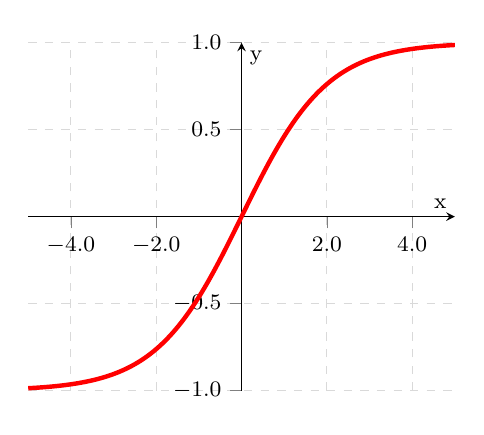
\begin{tikzpicture}
									\fontsize{8}{11}
									\begin{axis}[
											legend pos=north west,
											axis x line=middle,
											axis y line=middle,
											x tick label style={/pgf/number format/fixed,
																					/pgf/number format/fixed zerofill,
																					/pgf/number format/precision=1},
											y tick label style={/pgf/number format/fixed,
																					/pgf/number format/fixed zerofill,
																					/pgf/number format/precision=1},
											grid = major,
											width=70mm,
											height=6cm,
											grid style={dashed, gray!30},
											xmin=-5,     % start the diagram at this x-coordinate
											xmax= 5,    % end   the diagram at this x-coordinate
											ymin= -1,     % start the diagram at this y-coordinate
											ymax= 1,   % end   the diagram at this y-coordinate
											%axis background/.style={fill=white},
											xlabel=x,
											ylabel=y,
											tick align=outside,
											enlargelimits=false]
									% plot the stirling-formulae
									\addplot[domain=-5:5, red, ultra thick,samples=500] {2*(1/(1+e^-x))-1};
									% \addlegendentry{$f(x)=\frac{1}{1+e^{-5x}}$}
									\end{axis}
							\end{tikzpicture}
							\caption{graph of tanh function $f(x)={\frac{2}{1+e^{-x}}- 1}$ \label{sigmoid}}
						\end{figure}
					\end{center}
			\end{column}
		\end{columns}

		
	\end{frame}


% ----------------------------
% Decision Tree
% ----------------------------

	% Decision Tree
	\begin{frame}
		\frametitle{Choosing moves}
		\begin{figure}
			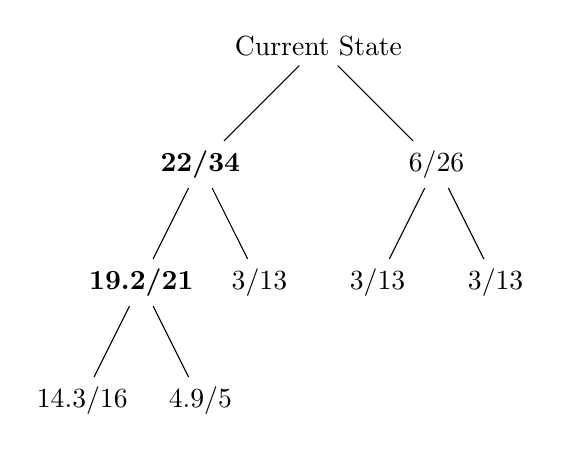
\begin{tikzpicture}[level distance=1.5cm,
				level 1/.style={sibling distance=3cm},
				level 2/.style={sibling distance=1.5cm}]
				\node {Current State}
					% left
					child { node {\bf 22/34}
						child {
							node {\bf 19.2/21} 
							child {node{14.3/16}}
							child {node{4.9/5}}
						}
						child {node {3/13}}
					}
					% right
					child {node {6/26}
					child {node {3/13}}
						child {node {3/13}}
					};
			\end{tikzpicture}
	\end{figure}
	\end{frame}

	% monte carlo
	\begin{frame}
		\frametitle{Monte Carlo Tree Search}

		
		\begin{figure}
			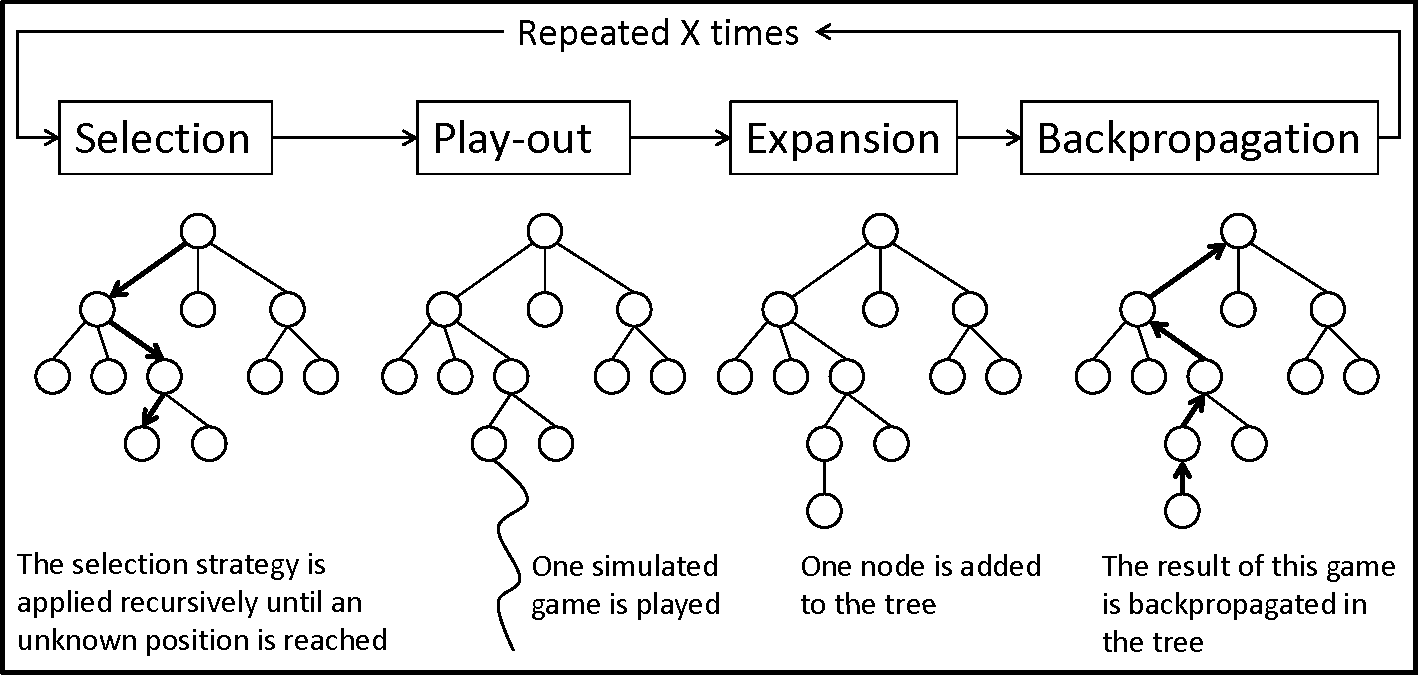
\includegraphics[width=110mm]{montecarlo.png}
			\caption{Diagram describing the MCTS process. Source: Winands et al. (\cite{winands_monte_2010})}
		\end{figure}
		% A grossly simplified algorithm:

		% \begin{itemize}
		% 	\item Generate a set of possible moves $m$ that can be made from some state
		% 	\item Choose random move $k \in m$.
		% 	\item Simulate a random, theoretical game from this;
		% 	\item Keep choosing random moves $n$ amount of times
		% 	\item after $n$ moves, evaluate using our neural network to make $x$!
		% 	\item Increment the number of simulations taken from $k = i$ 
		% 	\item Increment the chances of a good move from $k$ by $x$.
		% 	\item When satisfied, choose $k$ with the biggest $x/i$!
		% \end{itemize}

		% The intuition behind MCTS is that it leans towards better moves probablistically.
	\end{frame}
% ----------------------------
% Generating Agents
% ----------------------------

	% generating agents
	\begin{frame}
		\frametitle{Generating Agents}
		\begin{block}{Agent}
			An agent is a generated set of weights and biases for a neural network.
		\end{block}

		\begin{itemize}
			\item An initial agent would have a randomly generated set of weights and biases
			\item initial values range from -0.2 to 0.2.
		\end{itemize}
	\end{frame}

	% tournament
	\begin{frame}
		\frametitle{Tournament}
		\begin{enumerate}
			\item Generate a population of random agents (A population of 15 is used.)
			\item Make agents play each other
			\item Order agents by the amount of points scored
			\item The best few agents are chosen to stay on for the next tournament
			\item Make new agents from them
			\item The losers are destroyed
			\item Repeat step 2-6 with the new agents until satisfied
		\end{enumerate}
	\end{frame}

% ----------------------------
% Genetic Algorithms
% ----------------------------

	% crossover mechanism
	\begin{frame}
		\frametitle{Crossover Mechanism}

		\begin{figure}
			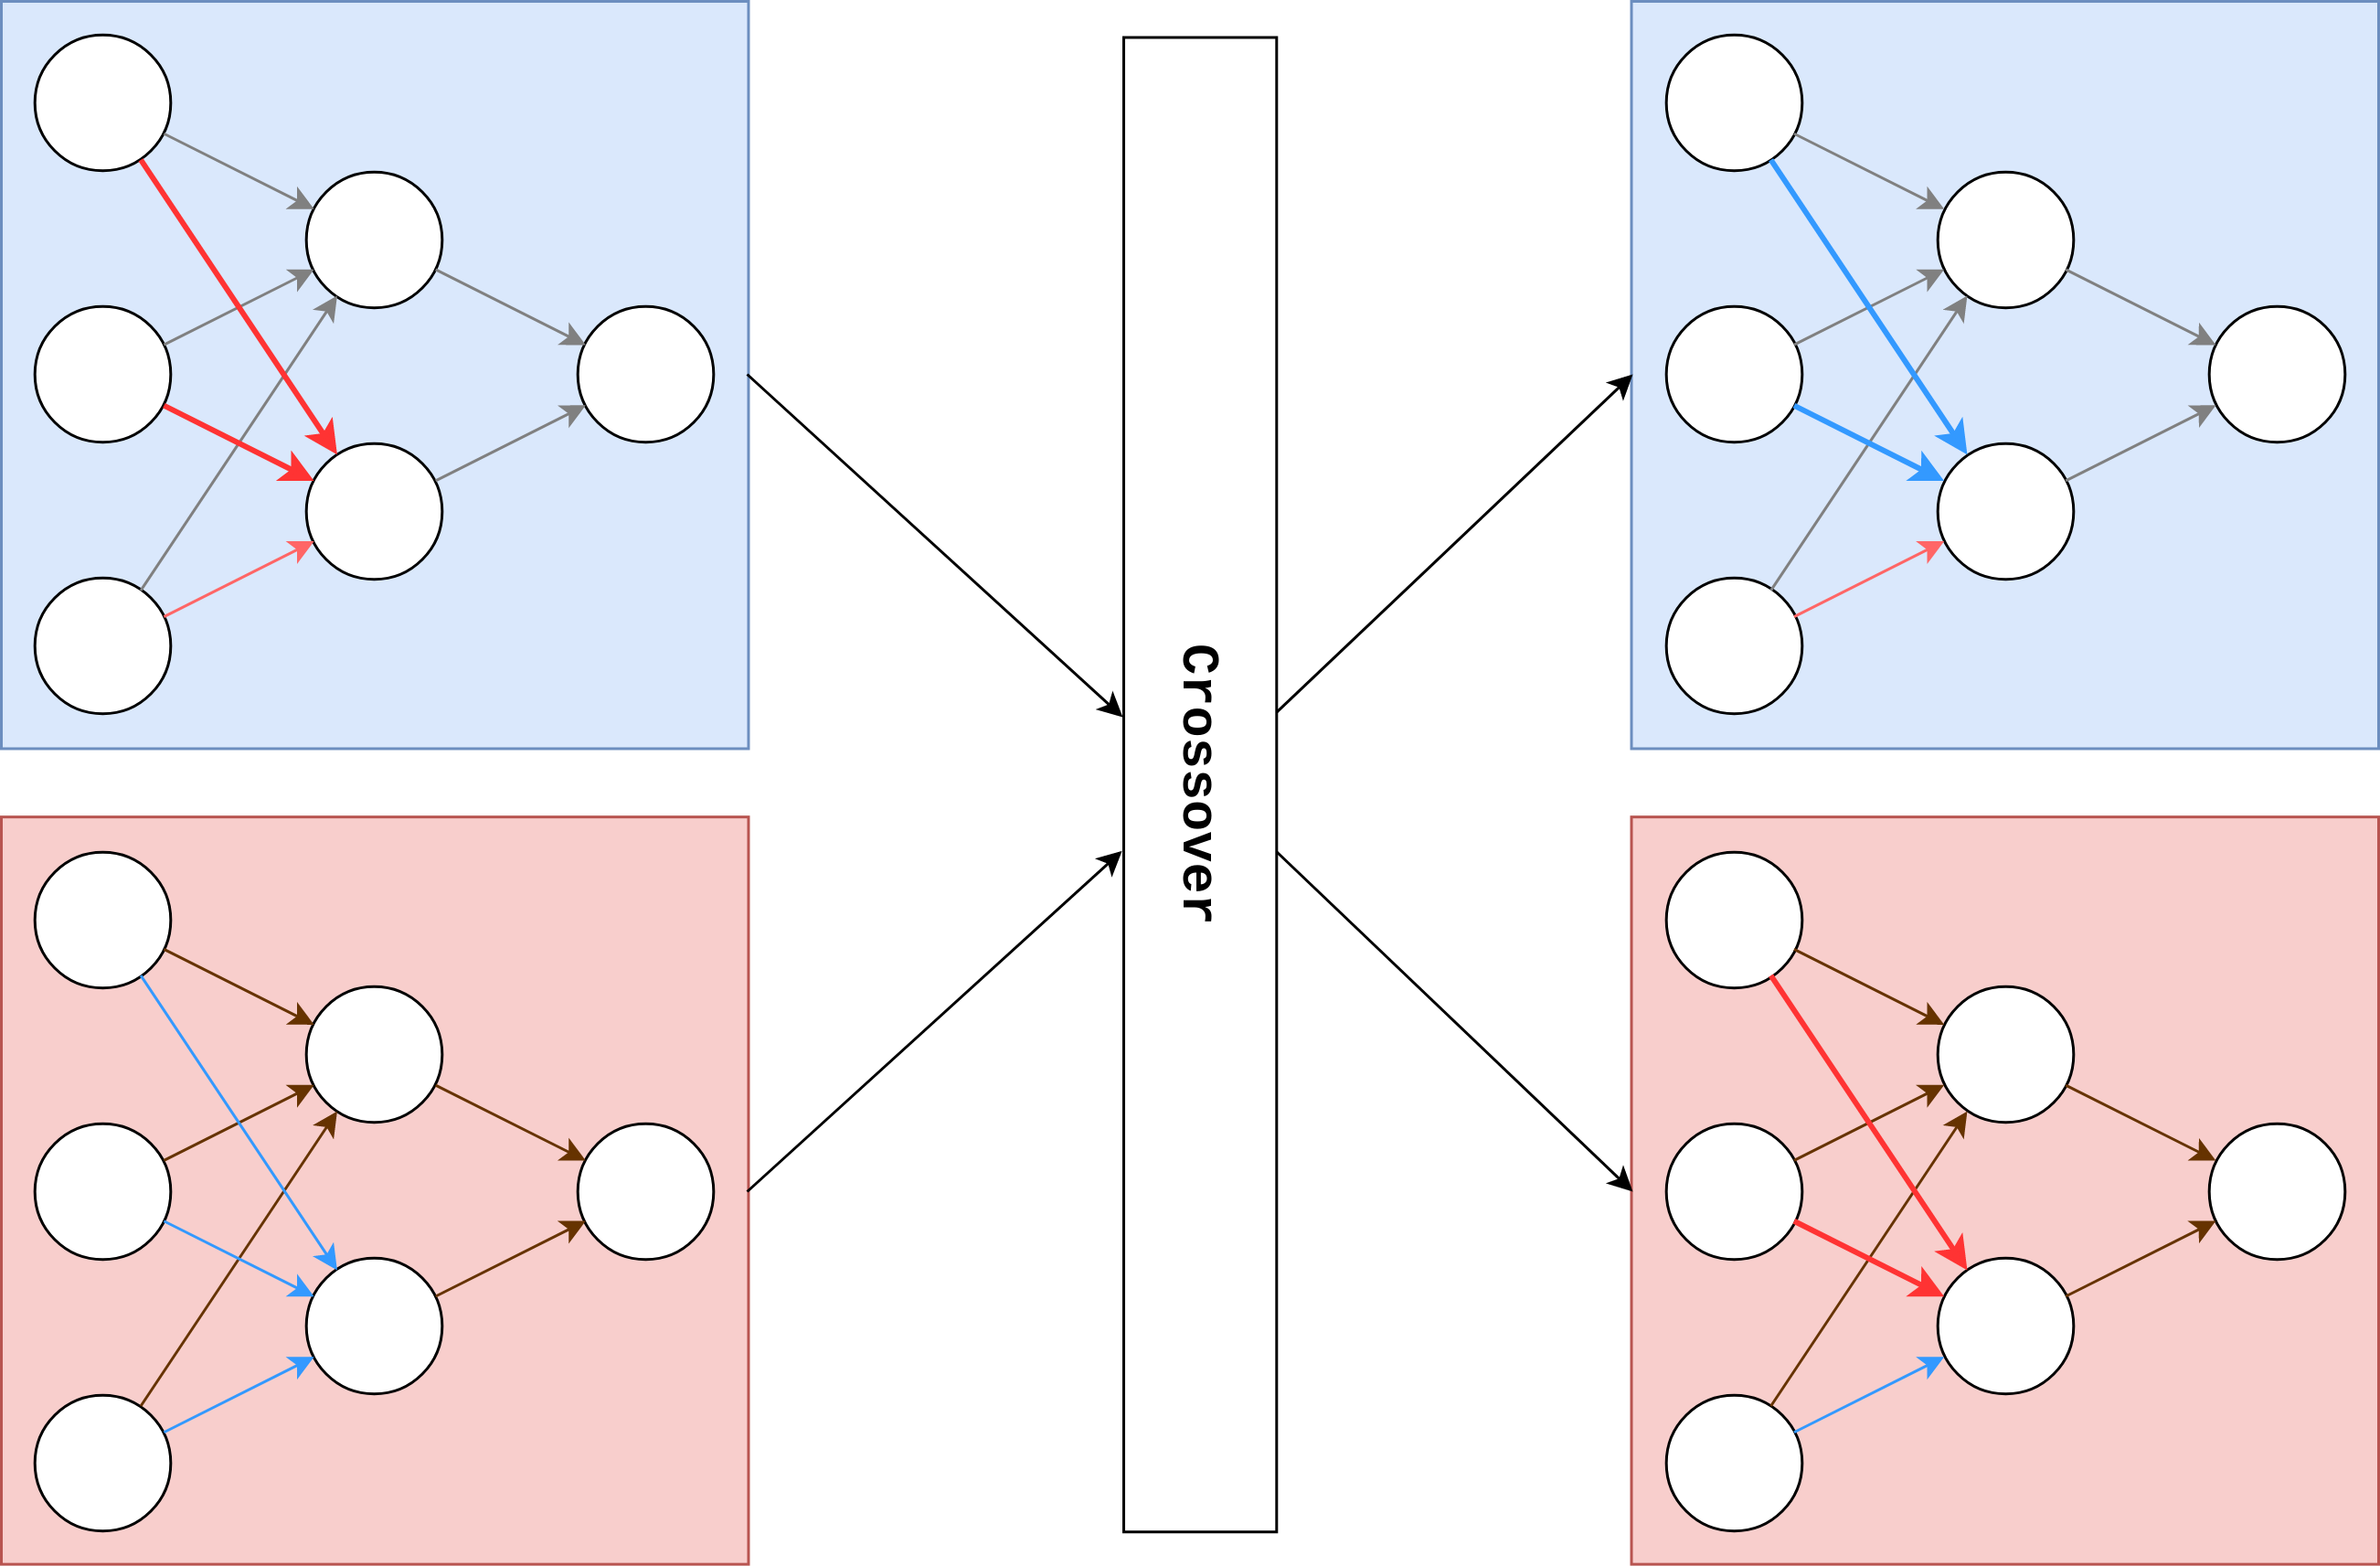
\includegraphics[width=80mm]{crossover.png}
			\caption{Offspring agents are created from a pair of parent agents.
			Each offspring is a reciprocal crossover of each other. A random hidden node is chosen, and influential inputs for that node are swapped between the two agents.}
		\end{figure}

		\begin{figure}
			% \begin{figure}
			% 		\LARGE
			% 	\begin{forest}
			% 		for tree={grow=north}
			% 		[	{
			% 			$O_{1} =$ [ 
			% 					{\color{red}1}
			% 					{\color{blue}7}
			% 					{\color{red}3}
			% 					{\color{blue}9}
			% 					{\color{red}5} 
			% 				], 
			% 				$O_{2} =$	[ 
			% 					{\color{blue}6}
			% 					{\color{red}2}
			% 					{\color{blue}8}
			% 					{\color{red}4}
			% 					{\color{blue}10} 
			% 				]
			% 			}
			% 			[
			% 				{
			% 					$P_{2} =$ [
			% 						{\color{blue}6}
			% 						{\color{blue}7}
			% 						{\color{blue}8}
			% 						{\color{blue}9}
			% 						{\color{blue}10}
			% 					]
			% 				}
			% 			]
			% 			[
			% 				{
			% 					$P_{1} =$[
			% 						{\color{red}1}
			% 						{\color{red}2}
			% 						{\color{red}3}
			% 						{\color{red}4}
			% 						{\color{red}5}
			% 					]
			% 				}
			% 			] 
			% 		]
			% 	\end{forest}
			% 	\vspace{10mm}
			% \end{figure}
		\end{figure}
		% for each layer's weights:
		%     n = number of weights and biases in a given layer
		%     index1 = random integer[0 to n]
		%     index2 = random integer[0 to n]
		%     if index2 < index1:
		%         swap index1 and index2's values
		%     Weights(child1) = $parent_{1}$[0 to index1] +  $parent_{2}$[index1 to index 2] + $parent_{1}$[index2 to n]
		%     Weights(child2) =  $parent_{2}$[0 to index1] + $parent_{1}$[index1 to index 2] +  $parent_{2}$[index2 to n]
				
	\end{frame}

	% mutation
	\begin{frame}
		\frametitle{Mutation}
		$WeightP$ is the current weight, $K$ represents the number of weights and biases in the neural network, and $m$ represents a random floating point in the range of [-1,1]:

			$$ WeightN = WeightP + \frac{m}{\sqrt{2 * \sqrt{K} }}$$

		Mutation influence is dependent on the number of weights in the system; The more weights in the network implies a less significant mutation.
	\end{frame}

% ----------------------------

% How to Evaluate
\begin{frame}
	\frametitle{Evaluation}
	% Your approach to solving the problem
	% How will I Judge the outcome of the work?
	\framesubtitle{How will I judge my outcome?}

	\begin{itemize}
		\item Measurements held to measure evolution progress
		\item Play final agent against agent from prior stages to indicate whether it has been learning
		\item Play against a randomly playing bot to see it is actually thinking
		\item Play against different move making algorithms (Vanilla MCTS, $\alpha \beta$ MiniMax)
		\item Also play against human players on popular checkers websites
	\end{itemize}
\end{frame}

% Current Progress
\begin{frame}
	\frametitle{Current Progress}
	% Your approach to solving the problem
	% How will I Judge the outcome of the work?
	\framesubtitle{What have I done already?}

	\begin{itemize}
		\item The initial set up is ready*
		\item It has been trained*
		\item It plays relatively well (anecdotally)
		\item Relatively ineffective at end game performances...
	\end{itemize}
\end{frame}

% Remaining Work
\begin{frame}
	\frametitle{Remaining Work}
	\framesubtitle{What do I still need to do?}
	% What did or will you accomplish?
	% What still needs to be done
	% \framesubtitle{A bit more information about this}
	\begin{itemize}
		\item * Squash potential bugs that could impede performance/provide false positives
		\item Experiment with different crossover and mutation mechanisms
		\item Optimise training (enforce threefold repetition)
		\item Train the system for a bit longer
		\item Measure the system's performance against other players
	\end{itemize}
\end{frame}

\begin{frame}
	\frametitle{Fin.}
	
	% What did or will you accomplish?
	% What still needs to be done
	% \framesubtitle{A bit more information about this}
	\begin{figure}
		\LARGE
	Any Questions?
	\end{figure}
\end{frame}

% References
\begin{frame}
	\frametitle{References}
	\framesubtitle{Nanos gigantum humeris insidentes}
	% What did or will you accomplish?


	
	{
		\tiny
		\bibliography{ref}
		\bibliographystyle{plain}
	}

	% \bibliography{ref}

	% What still needs to be done
	% \framesubtitle{A bit more information about this}
\end{frame}

\end{document}

% 

% \begin{wrapfigure}{l}{1 \textwidth}
%     % \begin{center}
%     \fontsize{16}{2}

%     \centering

%         \begin{tikzpicture}
%         \color{white}
%         \matrix (m) [matrix of nodes, nodes in empty cells, label skeleton, nodes={minimum size = 2cm}] {
%         & 31 &&30&&29&&28 \\
%         27 &&26&&25&&24&&\\
%         &23&&22&&21&&20\\   
%             19&&18&&17&&16&&\\
%         &15&&14&&13&&12\\
%         11&&10&&9&&8&&\\
%         &7&&6&&5&&4\\
%         3&&2&&1&&0\\
%         \bl &     & \bl &     & \bl &     & \bl &     \\
%             & \bl &     & \bl &     & \bl &     & \bl \\
%         \wh &     & \bl &     &     &     & \bl &     \\
%             &     &     & \wh &     & \bl &     & \wh \\
%         \wh &     & \wh &     &     &     & \wh &     \\
%             &     &     &     &     &     &     & \wh \\
%         \wh &     & \wh &     & \wh &     & \wh &     \\
%             & \wh &     & \wh &     & \wh &     & \wh \\
%         };
%         \foreach \row in {1, ..., 8} {
%         \foreach \col in {1, ..., 8} {
%             \pgfmathparse{Mod(\row + \col, 2) ? "black" : "red"}
%             \colorlet{squarebg}{\pgfmathresult}
%             \fitandstyle[background]{(m-cell-\row-\col)}{fill = squarebg}
%         }
%         }
%         \end{tikzpicture}
%     % \end{center}
  
% \end{wrapfigure}